\documentclass{exam}
%\documentclass[11pt,a4paper]{exam}
\usepackage{amsmath,amsthm,amsfonts,amssymb,dsfont}
\usepackage{ifthen}
\usepackage{enumerate}% http://ctan.org/pkg/enumerate
\usepackage{multicol}
\usepackage{graphicx}
\usepackage{float}

% Accumulate the answers. Unmodified from Phil Hirschorn's answer
% https://tex.stackexchange.com/questions/15350/showing-solutions-of-the-questions-separately/15353
\newbox\allanswers
\setbox\allanswers=\vbox{}

\newenvironment{answer}
{%
    \global\setbox\allanswers=\vbox\bgroup
    \unvbox\allanswers
}%
{%
    \bigbreak
    \egroup
}

\newcommand{\showallanswers}{\par\unvbox\allanswers}
% End Phil's answer


% Is there a better way?
\newcommand*{\getanswer}[5]{%
    \ifthenelse{\equal{#5}{a}}
    {\begin{answer}\thequestion. (a)~#1\end{answer}}
    {\ifthenelse{\equal{#5}{b}}
        {\begin{answer}\thequestion. (b)~#2\end{answer}}
        {\ifthenelse{\equal{#5}{c}}
            {\begin{answer}\thequestion. (c)~#3\end{answer}}
            {\ifthenelse{\equal{#5}{d}}
                {\begin{answer}\thequestion. (d)~#4\end{answer}}
                {\begin{answer}\textbf{\thequestion. (#5)~Invalid answer choice.}\end{answer}}}}}
}

\setlength\parindent{0pt}
%usage \choice{ }{ }{ }{ }
%(A)(B)(C)(D)
\newcommand{\fourch}[5]{
    \par
    \begin{tabular}{*{4}{@{}p{0.23\textwidth}}}
        (a)~#1 & (b)~#2 & (c)~#3 & (d)~#4
    \end{tabular}
    \getanswer{#1}{#2}{#3}{#4}{#5}
}

%(A)(B)
%(C)(D)
\newcommand{\twoch}[5]{
    \par
    \begin{tabular}{*{2}{@{}p{0.46\textwidth}}}
        (a)~#1 & (b)~#2
    \end{tabular}
    \par
    \begin{tabular}{*{2}{@{}p{0.46\textwidth}}}
        (c)~#3 & (d)~#4
    \end{tabular}
    \getanswer{#1}{#2}{#3}{#4}{#5}
}

%(A)
%(B)
%(C)
%(D)
\newcommand{\onech}[5]{
    \par
    (a)~#1 \par (b)~#2 \par (c)~#3 \par (d)~#4
    \getanswer{#1}{#2}{#3}{#4}{#5}
}

\newlength\widthcha
\newlength\widthchb
\newlength\widthchc
\newlength\widthchd
\newlength\widthch
\newlength\tabmaxwidth

\setlength\tabmaxwidth{0.96\textwidth}
\newlength\fourthtabwidth
\setlength\fourthtabwidth{0.25\textwidth}
\newlength\halftabwidth
\setlength\halftabwidth{0.5\textwidth}

\newcommand{\choice}[5]{%
\settowidth\widthcha{AM.#1}\setlength{\widthch}{\widthcha}%
\settowidth\widthchb{BM.#2}%
\ifdim\widthch<\widthchb\relax\setlength{\widthch}{\widthchb}\fi%
    \settowidth\widthchb{CM.#3}%
\ifdim\widthch<\widthchb\relax\setlength{\widthch}{\widthchb}\fi%
    \settowidth\widthchb{DM.#4}%
\ifdim\widthch<\widthchb\relax\setlength{\widthch}{\widthchb}\fi%

% These if statements were bypassing the \onech option.
% \ifdim\widthch<\fourthtabwidth
%     \fourch{#1}{#2}{#3}{#4}{#5}
% \else\ifdim\widthch<\halftabwidth
% \ifdim\widthch>\fourthtabwidth
%     \twoch{#1}{#2}{#3}{#4}{#5}
% \else
%      \onech{#1}{#2}{#3}{#4}{#5}
%  \fi\fi\fi}

% Allows for the \onech option.
\ifdim\widthch>\halftabwidth
    \onech{#1}{#2}{#3}{#4}{#5}
\else\ifdim\widthch<\halftabwidth
\ifdim\widthch>\fourthtabwidth
    \twoch{#1}{#2}{#3}{#4}{#5}
\else
    \fourch{#1}{#2}{#3}{#4}{#5}
\fi\fi\fi}

\begin{document}
\begin{titlepage}
    \begin{center}
        \vspace*{1cm}
            
        \Huge
        \textbf{Statistics MCQ Question Bank} \\
        
       
            
        \vspace{0.5cm}
        \LARGE
        First Paper \\

            
        \vspace{1.5cm}
            
        \textbf{Abdullah Al Mahmud}
            
        \vfill
            
            \textbf{Last updated: \today}
        \vspace{0.8cm}
        
             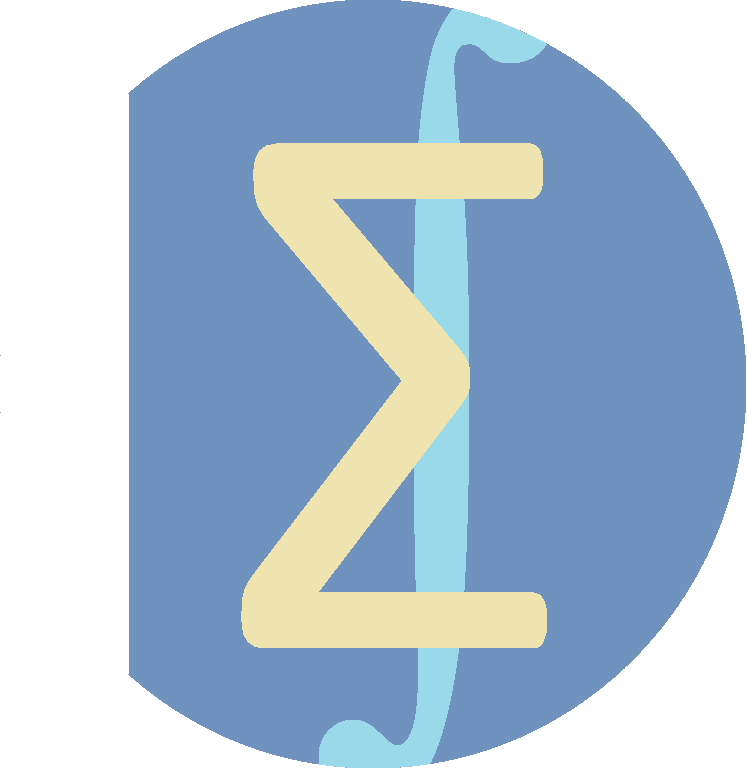
\includegraphics[width=1cm]{logo}
            
        \Large
        www.statmania.info\\
            
    \end{center}
\end{titlepage}


\begin{questions}

\section{Basic Concept of Statistics}

\question \textbf{Who is known as the Father of modern statistics?}
\choice{P.C. Mahalanobis}{Kazi Motaher Hossain}{Karl Pearson}{R.A. Fisher}{d}

\question \textbf{Which of the following is correct?}
\choice{$\displaystyle \sum_{i=1}^{20} cx_i = nc \sum_{i=1}^{20} x_i$}{$\displaystyle \sum_{i=1}^{20} cx_i = nc \sum_{i=1}^{20} x_i$}{$\displaystyle \sum_{i=1}^{20} cx_i = c \sum_{i=1}^{20} x_i$}{$\displaystyle \sum_{i=1}^{20} cx_i = c^2 \sum_{i=1}^{20} x_i$}{b}

\question \textbf{Which cannot be performed using Univariate data?}
\choice{Central tendency}{Dispersion}{Skewness}{Regression}{d}

\question \textbf{Cities ranked according to habitability level show -- measurement scale}
\choice{Nominal}{Ratio}{Interval}{Ordinal}{d}

\question \textbf{Which is not an example of shift of scale?}
\choice{$y_i = \frac{x_i}{a}$}{$y_i = cx_i$}{$y_i = x_i-2$}{$y_i = \frac{cx_i}{d}$}{a}

\question \textbf{If $\displaystyle \sum_{i=1}^{20} x_i^2=20$ and $\displaystyle \sum_{i=1}^{20} x_i=30$, what is the value of $\displaystyle \sum_{i=1}^{20} x_i^2 + \sum_{i=1}^{20} x_i + 100$?}
\choice{130}{200}{150}{2130}{c}

\question \textbf{A subset of a population is called--}
\choice{Constant}{Variable}{Sample}{Scale}{c}

\question \textbf{How many measurement scales are there?}
\choice{2}{3}{4}{5}{c}

\question \textbf{Which of the following is a continuous variable?}
\choice{Number of goals}{Natural number}{Summation of Fibonacci series}{Success rate}{d}

\question \textbf{In which scale of measurement, zero is regarded as true zero?}
\choice{Nominal scale}{Interval scale}{Ratio scale}{Ordinal scale}{c}

\question \textbf{Which is a discrete variable?}
\choice{Weight}{Amount of rainfall}{Distance}{Grade in a subject}{d}

\question \textbf{$If x_1=2, x_2=-3, x_3=7$, and $x_4=12, \displaystyle \sum_{i=1}^4 x_i^2=?$}
\choice{26}{106}{206}{216}{c}

\question \textbf{$If x_1=2, x_2=3, x_3=4, x_4=6$, and $x_5=5, \displaystyle \sum_{i=1}^4 x_i^2=?$}
\choice{80}{87}{90}{105}{c}

\question \textbf{Capital and profit belong to a variable which is--}

i. Bivariate \\
ii. Quantitative \\
iii. Qualitative

\textbf{Which one is correct?}

\choice{i and ii}{i and iii}{ii and iii}{i, ii and iii}{a}

\question \textbf{Which one falls in the category of interval scale?}
\choice {Temperature}{Speed}{Distance}{Film rating}{a}

\question \textbf{In which scale of measurement, zero is regarded as true zero?}
\choice{Nominal scale}{Interval scale}{Ratio scale}{Ordinal scale}{c}

\question \textbf{Which is a discrete variable?}
\choice{Weight}{Amount of rainfall}{Distance}{Grade in a subject}{d}

\question \textbf{Which one is product of square?}
\choice {$\prod x_i^2$}{$(\prod x_i)^2$}{$\sum x_i^2 \times \sum x$}{$\sum x_i^2$}{a}

\question \textbf{For which variable, determining number of terms is not possible?}
\choice{Discrete variable}{Continuous variable}{Quantitative variable}{Qualitative variable}{b}

\textbf{Answer the next three question based on the following information.}

\textbf{A farmer collects growth (in cm) of 10 plants in a month and finds that \\ $\sum x_i = 7$ and $\sum x_i^2=15$}

\question \textbf{What is the value of $\sum (x_i+4)$?}
\choice{23}{47}{22}{11}{b}

\question \textbf{If $\displaystyle x_1=2, x_2=3, x_3=5, x_4=7$ and $\displaystyle y_1=3, y_2=4, y_3=5, y_4=8; 
 \sum_{i=2}^4 x_iy_i=?$}
\choice{14}{201}{93}{117}{c}


\question \textbf{From the following table, $\displaystyle \sum_{i=1}^4 x_iy_i=?$}

\begin{table}[h]
\centering
\begin{tabular}{c|c|l|c|l}
X & 1  & 5  & 3 & 2  \\ \hline
Y & 20 & 12 & 3 & 14
\end{tabular}
\end{table}

\choice{14}{201}{99}{109}{c}

\question \textbf{What is the value of $\sum (x_i-4)^2$?}
\choice{23}{135}{484}{119}{d}

\question \textbf{If the square of summation is subtracted the sum of square, the value is - }
\choice{-8}{34}{8}{-34}{d}

\question \textbf{Which one is not an example of ratio scale?}
\choice{Room no.}{Income}{Number of accidents}{Weight}{a}

\question \textbf{Which one is discrete?}
\choice{Weight}{Amount of rainfall}{Temperature}{No. of member in a family}{d}

\question \textbf{Which type of scale of measurement are religion and blood group?}
\choice{Interval}{Ratio}{Nominal}{Ordinal}{c}

%-----------------------------------Section 2

\section{Collection, Organization, and Presentation of Data}

%-----------------------------------Section 2

\question \textbf{How many sources of data are there?}
\choice{5}{4}{3}{2}{d}

\question \textbf{What is the raw material of research?}
\choice{Data}{Theory}{Graph}{Mean}{a}

\question \textbf{Data obtained through direct observation is called--}
\choice{Primary data}{Secondary data}{Original Data}{Informal data}{a}

\textbf{Answer the next THREE questions based on the following information}

Radius of 80 trees are recorded and this frequency distribution is constructed.

\begin{table}[H]
\centering
\begin{tabular}{c|c|c|c|c}
\begin{tabular}[c]{@{}c@{}}Radius (cm)\end{tabular} & 0-10 & 10-20 & 20-30 & 30-40 \\ \hline
No. of Trees & 20 & 15 & 21 & 24
\end{tabular}
\end{table}

\question \textbf{How many trees have radius between 10 and 30?}
\choice{30}{15}{36}{21}{c}

\question \textbf{How many trees have radius at least 20?}
\choice{44}{45}{24}{21}{b}

\question \textbf{What percent of trees have radius between 20 and 40?}
\choice{44\%}{56\%}{46\%}{53\%}{a}

\question \textbf{Which formula is used to find angles for Pie Chart?}
\choice{$\theta_i = \frac{f_i}{N}\times 100$}{$\theta_i = \frac{f_i}{100}\times 360$}{$\theta_i = \frac{f_i}{N}\times 360$}{$\theta_i = \frac{f_i}{N-1}\times 360$}{c}

\question \textbf{Who invented Stem and Leaf plot?}
\choice{Karl Pearson}{R.A. Fisher}{David Cox}{John Tukey}{d}

\question \textbf{If all the rats in Sylhet is a population, all the rats in Sylhet Airport is --}
\choice{Data}{Sample}{Statistics}{Frequency}{b}

\question \textbf{Which rule is suggested by H.G. Sturges for determining number of class (k)?}
\choice{$K=1+3.322logN$}{$K=1+3.222logN$}{$K=1-3.222logN$}{$K=1+2.332logN$}{a}

\question \textbf{To show runs per over in a cricket match, which diagram can be used?}
\choice{Histogram}{Bar Diagram}{Ogive}{Frequency polygon}{b}

\section{Measures of Central Tendency}

%-----------------------------------------------------------------------
\subsection{General Questions}
%-----------------------------------------------------------------------

\question \textbf{Which statement is correct}
\choice{Quartiles are well defined}{Outliers affect Median}{Median is always present in data}{Quadratic mean is widely used}{a}

\question \textbf{If a value is zero, which measure is not usable?}
\choice{Arithmetic Mean}{Harmonic Mean}{Geometrtic Mean}{Mode}{c}

\question \textbf{How many measure of central tendency are there?}
\choice{2}{3}{4}{5}{d}

\question \textbf{Which measure of central tendency is suitable for qualitative variable?}
\choice{Arithmetic Mean}{Harmonic Mean}{Quadratic Mean}{Mode}{d}

\question \textbf{In presence of negative values, which measure is not usable?}
\choice{Arithmetic Mean}{Geometric Mean}{Quadratic Mean}{Harmonic Mean}{b}

\question \textbf{Inappropriate for algebraic analysis--}

i. Median \\
ii. Mode \\
iii. Geometric Mean

Which one is true?

\choice{i}{ii}{i \& ii}{ii \& iii}{c}

\textbf{Answer the next two questions based on the following information}


  \begin{table}[h]
\centering
\begin{tabular}{cccccc}
Accident     & 4 & 6 & 7 & 8 & 9\\ \hline
Frequency & 2   & 0    & 4     & 5     & 1   
\end{tabular}
\end{table}
\question \textbf{Fifth Decile is --}
\choice{0}{8.5}{7.5}{8}{c}

\question \textbf{Which of the following is mode?}
\choice{4}{8}{0}{7}{b}

\question \textbf{Which measure gives a value from within the values?}
\choice{Arithmetic Mean}{Geometric Mean}{Median}{Mode}{d}

\question \textbf{Which one is not a proper measure of central tendency?}
\choice{2nd Quartile}{Third Decile}{3rd Quintile}{110th Percentile}{d}

\question \textbf{Which one is smallest?}
\choice{$\displaystyle \sum_{i=1}^n (X_i-Median)^2$}{$\displaystyle \sum_{i=1}^n (X_i-\bar X)^2$}{$\displaystyle \sum_{i=1}^n (X_i-\sigma)^2$}{$\displaystyle \sum_{i=1}^n (X_i-Mode)^2$}{a}

\question \textbf{Which measure is not used in determining skewness?}
\choice{Arithmetic Mean}{Geometric Mean}{Median}{Mode}{b}

\question \textbf{When is the relationship $AM = HM = GM$ true?}
\choice {All values are equal}{The values form a geometric progression}{ The values form an arithmetic progression}{All values are distinct}{a}

\question \textbf{In the presence of outlier(s), which measure of central tendency is suitable?}
\choice {Arithmetic mean}{Median}{Quadratic mean}{Power mean}{b}

\question \textbf{If a rate is defined as $R = \frac cd$, where c is constant, then which measure is perfect?}
\choice {Weighted arithmetic mean}{Harmonic mean}{Quadratic mean}{Weighted geometric mean}{b}

\question \textbf{Which measure might have more than one value?}
\choice{Arithmetic mean}{Geometric mean}{Quadratic mean}{Mode}{d}

\question \textbf{Which relationship is correct?}
\choice{$AM \times GM = HM^2$}{$AM \times HM = GM^2$}{$AM \times HM = GM^3$}{$AM \div GM = HM^2$}{b}

\question \textbf{With negative observations, which cannot be used}

i. Arithmetic Mean \\
ii. Geometric Mean \\
iii. Harmonic Mean

\textbf{Which one is correct?}

\choice{i and ii}{i and iii}{ii and iii}{i, ii and iii}{c}

%---------------------------------------------------------
\subsection{Arithmetic Mean}
%---------------------------------------------------------

\question \textbf{Arithmetic Mean is --}

i. Rigidly defined \\
ii. Unaffected by sample fluctuation \\
iii. Suitable for algebraic analysis

\textbf{Which one is correct?}

\choice{i and ii}{i and iii}{ii and iii}{i, ii and iii}{b}

\question \textbf{Arithmetic Mean of first 25 natural numbers is --}
\choice{12}{13}{14}{26}{b}

\question \textbf{Arithmetic Mean of two numbers is 25. If a number is 40, what is the other number?}
\choice{40}{50}{25}{10}{d}

\question \textbf{Number of students in two classes are 50 and 55 and their combined arithmetic mean (AM) of marks is 82. If AM of the first class is 75, what is the AM of the other class? }
\choice{88.36}{88.40}{84.55}{78.33}{a}

\question \textbf{The summation of deviation of each value from their arithmetic mean is --}
\choice{0}{1}{2}{4}{a}

\question \textbf{For grouped data, which formula is correct for Arithmetic Mean?}
\choice{$\displaystyle \bar X = \frac{\sum f_ix_i}{\sum f_i}$}{$\displaystyle \bar X = \frac{\sum x_i}{N}$}{$\displaystyle \bar X = \frac{\sum f_ix_i}{n}$}{$ \displaystyle\bar X = \frac{\sum f_i}{N}$}{a}

\question \textbf{Arithmetic mean of the series 2, 12, 22, $\cdots$, 92 is--}
\choice{45}{46}{47}{55}{c}

\question \textbf{What is the arithmetic mean of first n odd natural numbers?}
\choice{$\frac{n+1}{n}$}{n}{n+1}{$\frac{n+1}{2}$}{b}

\question \textbf{What is the arithmetic mean of first n even natural numbers?}
\choice{$\frac{n+1}{2}$}{$n+1$}{$n$}{$\frac{n-1}{2}$}{b}

\question \textbf{The arithmetic mean of first n natural numbers-}
\choice {$\frac{n}{2}$}{$\frac{n+1}{2}$}{$\frac{n^2}{2}$}{$\frac{n^2-1}{2}$}{b}

\question \textbf{Arithmetic means of three groups having equal no. of items are 30, 32, and 34. What is the combined mean?}
\choice{30.33}{32.67}{32.00}{33.00}{c}

%--------------------------------------------
\subsection{Harmonic Mean}

%--------------------------------------------

\question \textbf{A rate is defined as $R = \frac c d;$  c and d are arbitrary numbers. If c is constant, which mean is used?}

\choice{Arithmetic Mean}{Geometric Mean}{Harmonic Mean}{Weighted Geometric Mean}{c}

\question \textbf{A rate is defined as $R = \frac c d;$  c and d are arbitrary numbers. If d is constant, which mean is used?}

\choice{Arithmetic Mean}{Geometric Mean}{Harmonic Mean}{Weighted Geometric Mean}{a}

\question \textbf{A rate is defined as $R = \frac c d;$  c and d are arbitrary numbers. If neither c or d is constant, which mean is used?}

i. Weighted Arithmetic Mean \\
ii. Weighted Harmonic Mean \\
iii. Harmonic Mean

\textbf{Which one is correct?}

\choice{i and ii}{i and iii}{ii and iii}{i, ii and iii}{a}

\choice{Arithmetic Mean}{Geometric Mean}{Harmonic Mean}{Weighted Geometric Mean}{c}

\question \textbf{Which is the respresentation of Harmonic Mean?}
\choice{Mean of Reciprocal}{Reciprocal of Mean}{Reciprocal of Mean of Reciprocal}{None of the above}{c}
%--------------------------------------------
\subsection{Geometric Mean}

%--------------------------------------------

\question \textbf{Which data set is suitable for Geometric Mean?}
\choice{$1,-1,2,4,6,7$}{$1,2,4,8,16,32$}{$0,1,2,3,4,6$}{$1,1,2,3,4,4,5$}{b}

\subsection{Mode}

\question \textbf{Which of the following may be used to determine mode?}
\choice{Histogram}{Frequency Curve}{Ogive}{Frequency Polygon}{a}

\subsection{Median}

\question \textbf{Median can be determined from the--}
\choice{Histogram}{Frequency curve}{Ogive}{Pie Chart}{c}

\textbf{Answer the next two (2) questions based on the following information}

\begin{table}[h]
\centering
\begin{tabular}{c|c|c|c|c|c|c}
Class                                                           & $\le 20$ & 20-25 & 25-50 & 50-60 & 69-70 & $\ge 70$ \\ \hline
Frequency                                                       & 5        & 10    & 10    & 7     & 5     & 3        \\ \hline
\begin{tabular}[c]{@{}c@{}}Cumulative \\ Frequency\end{tabular} & 5        & 15    & 25    & 32    & 37    & 40      
\end{tabular}
\end{table}

\question \textbf{How many values are between 20 and 70?}
\choice{20}{32}{35}{37}{b}

\question \textbf{Which one is the median class?}
\choice{20-25}{25-50}{50-60}{60-70}{b}

\subsection{Partition Values}

\textbf{Answer the next two questions as per the following information.}

42 44 59 64 70 72 74 91 94 are 9 values.

\question \textbf{What is the 50th percentile?}
\choice {64}{70}{72}{71}{b}

\question \textbf{Below which value lie 70 percent values?}
\choice {42}{44}{59}{74}{d}

\question \textbf{Above which value lie 30\% observations?}
\choice{3rd Quartile}{Median}{30th Percentile}{70th percentile}{d}


\section{Measures of Dispersion}

\question \textbf{Which of the following is the best measure of dispersion?}
\choice{Range}{Mean deviation}{Standard deviation}{Coefficient of variation}{c}

\question \textbf{What is the minimum possible value of standard deviation?}
\choice{$\infty$}{-1}{0}{1}{c}

\question \textbf{For two values, range is found to be 8. What are the values of mean deviation and standard deviation}
\choice{(2,4)}{(4,4)}{(4,8)}{(8,8)}{a}

\question \textbf{What is the standard deviation of first 10 natural numbers?}
\choice{2.87}{3.02}{0}{2.78}{a}

\question \textbf{Which measure is unit-free?}
\choice{Range}{Mean deviation}{Standard deviation}{Coefficient of variation}{d}

\section{Moments, Skewness, and Kurtosis}

\subsection{Moments}

\question \textbf{Which is not a type of Moments}
\choice{Central Moments}{Raw Moments}{Corrected Moments}{Rectified Moments}{d}

\question \textbf{The second moment around w is --}
\choice{$\frac{\sum (x_i-\bar x)^n}{w}$}{$\frac{\sum (x_i-\bar x)^2}{w}$}{$\frac{\sum (x_i-w)^2}{n}$}{$\frac{\sum (x_i-w)^n}{2}$}{a}

\question \textbf{Which quantity uniquely characterizes a distribution?}
\choice{Median}{Quantile}{Moments}{Trend}{c}

\textbf{Which one is correct?}

\choice{i and ii}{i and iii}{ii and iii}{i, ii and iii}{d}

\question \textbf{Which can be used to measure dispersion?}
\choice{$\mu_2'$}{$\mu_1$}{$\mu_2$}{$\mu_1'$}{c}

\question \textbf{The formula of coefficient of variance (CV) is --}
\choice{$\frac{\sqrt{\mu_2}}{n}\times 100$}{$\frac{\mu_2}{\mu_1}\times 100$}{$\frac{\sqrt{\mu_2}}{\bar x}\times 100$}{$\frac{\mu_3}{\sigma}\times 100$}{c}

\question \textbf{First moment around zero is --}
\choice{0}{1}{-1}{Arithmetic Mean}{d}

\question \textbf{Which might have a negative value?}
\choice{$\mu_4$}{$\mu_3$}{$\mu_2'$}{$\mu_2$}{b}

\question \textbf{2nd Central Moment is --}
\choice{$\mu_2-\mu_1'$}{$\mu_2+\mu_1'$}{$\mu_2-\mu_1'^2$}{$\mu_2'-\mu_1'^2$}{d}

\question \textbf{First central moment is equal to --}
\choice{1}{0}{-1}{$\bar x-a$}{b}

\question \textbf{First moment around a is equal to --}
\choice{1}{0}{-1}{$\bar x-a$}{d}

\question \textbf{The first raw moment about 3 is -5. What is the value of arithmetic mean?}
\choice{2}{-2}{0}{8}{b}

\question \textbf{Moments can be--}

i. positive \\
ii. not negative \\
iii. positive or negative

\textbf{Which one is correct?}

\choice{i and ii}{i and iii}{ii and iii}{i, ii and iii}{b}

%------------------------------------------------------------------------------
\subsection{Skewness}
%------------------------------------------------------------------------------

\question \textbf{The following graph is an example of --}

\begin{center}
   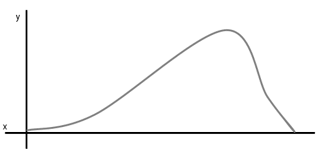
\includegraphics[width=0.2\textwidth]{../img/neg_skew.png}
\end{center}

\choice{Positive Skew}{Negative Skew}{No Skew}{Not detectable}{a}

\question \textbf{Characteristics of a skewed distributon are --}

i. $Mean \ne Median \ne Mode$ \\
ii. Differences of upper and lower quartiles from median are unequal\\
iii. Frequency curve is asymmetric

\question \textbf{In a distribution, $\mu_2=25, \mu_3=20$, and $\mu_4=2200$; the distribution is --}
\choice{Negativelky skewed}{leptokurtic}{Platykurtic}{Symmetric}{b}

\question \textbf{For a data, $Q_3=41.6, Q_1=17.2, Median = 29, \& AM = 30$; What is Coefficient of skewness?}
\choice{24.4}{1}{0.03}{29.45}{d}

\question \textbf{In case of positive skewness, which one is correct?}
\choice{$Mean>Median>Mode$}{$Mean<Median<Mode$}{$Mean=Median=Mode$}{$Mean>Median<Mode$}{a}

\question \textbf{For a symmetrical distribution, $\beta_1=$}
\choice{1}{-1}{0}{3}{c}

\question \textbf{$\sqrt{\beta_1}=-0.23$ implies--}
\choice{Left Skew}{Symmetry}{Right Skew}{Mesokurtic}{a}

\question \textbf{First 3 moments about 2 are 1, 2 and 8, respectively. What is the arithmetic mena?}
\choice{1}{2}{3}{4}{c}

\question \textbf{What is the second central moments of first 10 natural numbers?}
\choice{9.90}{9.09}{8.25}{5.67}{c}

\question \textbf{Frequencies of higher values are smaller in -- distribution}
\choice{Positively skewed}{Negatively skewed}{Symmetric}{Mesokurtic}{a}

\question \textbf{Which formula is correct for determining skewness?}
\choice{$\gamma_1 = \sqrt{\frac{\mu_3^2}{\mu_2^3}}$}{$\gamma_1=\sqrt{\beta_1^2}$}{$\gamma_1 = \sqrt{\frac{\mu_3}{\mu_2^3}}$}{$\frac{\mu_2}{\sqrt{\mu_3^2}}$}{a}

\subsection{Kurtosis}

\question \textbf{How many types of kurtosis are there?}
\choice{2}{3}{4}{5}{b}

\question \textbf{The standard deviation of a mesokurtik distribution is 2. What is the value of the 4th central moment?}
\choice{4}{8}{16}{48}{d}

\question \textbf{$\beta_2 = \sqrt 9$ implies data are--}
\choice{Leptokurtic}{Platykurtic}{Mesokurtic}{Symmetric}{c}

\question \textbf{For a mesokurtik distribution, $\beta_2 = --$}
\choice{0}{-3}{3}{1}{c}

\subsection{Misc}

\question \textbf{Which is not used in constructing Box \& Whisker Plot?}
\choice{Mode}{$X_L$}{$Q_1 \& Q_3$}{$Q_1, Q_2 \& Q_3$}{a}

\question \textbf{In a symmatric distribution--}

i. Arithmetic Mean = Mode = Median \\
ii. $Q_2-Q_1 = Q_3-Q_2$  \\
iii. $Q_1-X_L = X_H-Q_3$

Which one is true?

\choice{i \& ii}{ii \& iii}{i \&iii}{i, ii \&iii}{d}

\question \textbf{Which is not included in five number summary?}
\choice{Arithmetic Mean}{$X_H$}{$Q_2$}{$Q_3$}{a}

\section{Correlation and Regression}


%------------------------------------------------------------------------------
\section{Time Series}
%------------------------------------------------------------------------------

\question \textbf{A linear trend goes along a -- }
\choice{a curved line}{a wave}{straight line}{circle}{a}

\textbf{Answer the next THREE questions based on the following information}

\begin{table}[h]
\begin{tabular}{c|cccccccc}
Year & 2016 & 2017 & 2018 & 2019 & 2020 & 2021 & 2022 & 2023 \\ \hline
USD Exchange Rate & 78.35 & 79.49 & 82.87 & 83.26 & 84.60 & 84.37 & 85.80 & 106.70
\end{tabular}
\caption{\label{usdrate}Source--Investing.com}
\end{table}

\question \textbf{What is the second value of semi-average method?}
\choice{85.40}{90.37}{91.73}{89.78}{b}

\question \textbf{What kind of a trend do the data have?}
\choice{Upward}{Downward}{Both upward \& downward}{No trend}{a}

\question \textbf{Which component of time series is visible in the later part of the data?}
\choice{Seasonal Variation}{General Trend}{Irregular Variation}{Cyclic Variation}{c}

\question \textbf{Time Series has how many components?}
\choice{2}{3}{4}{5}{c}

\question \textbf{Which component involves period more than one (01) year?}
\choice{Seasonal Variation}{Cyclic Variation}{Irregular Variation}{Random Variation}{b}

\question \textbf{Which one is not a component of Time Series}
\choice{Seasonal Variation}{Cyclic Variation}{General Trend}{Regular Variation}{d}

\question \textbf{A company is constantly getting greater revenue than previous year; this is--}
\choice{Seasonal Variation}{General Trend}{Irregular Variation}{Cyclic Variation}{b}

\question \textbf{Which is not a method of finding general trend?}
\choice{Graphical Method}{Moving Average}{Semi-Average}{Moving Median}{d}

\textbf{Answer the next two questions based on the following table:}

  \begin{table}[h]
\centering
\begin{tabular}{ccccccc}
Year     & 2007 & 2008 & 2009 & 2010 & 2011 & 2012\\ \hline
Sales & 5   & 35    & 34     & 40     & 42  & 204 
\end{tabular}
\end{table}

\question \textbf{In Semi-Average method, what is the 2nd average?}
\choice{74}{24.67}{95.33}{28}{c}

\question \textbf{What is the last  value of 3-yearly moving average?}
\choice{93.55}{95.53}{95.33}{59.33}{c}

\question \textbf{Which component of time series is affected by economic changes due to war?}
\choice{Trend}{Seasonal Variation}{Irregular Variation}{Cyclic Variation}{c}

\question \textbf{Demand for warm clothes is higher in winter season ans less in summer. Which component of time series deals with this change?}
\choice{Trend}{Seasonal Variation}{Irregular Variation}{Cyclic Variation}{b}

\question \textbf{Death rates of a country for 7 years are given below:}

\begin{table}[H]
\centering
\begin{tabular}{c|c|c|c|c|c|c|l}
Year & 2009 & 2010 & 2011 & 2012 & 2013 & 2014 & 2015 \\ \hline
Rate & 5    & 7    & 6    & 8    & 7    & 12   & 13  
\end{tabular}
\end{table}

\textbf{In semi-average method, which year will be excluded?}
\choice{2012}{2013}{ 2015}{2009}{b}

\question \textbf{Which component of time series represents a natural disaster?}
\choice{Seasonal Variation}{General Trend}{Irregular Variation}{Cyclic Variation}{c}

\question \textbf{How many models of time series are there to combine the components?}
\choice{2}{3}{4}{5}{a}

%-------------------------------------------------------------------------------
\section{Published Statistics in Bangladesh}
%-------------------------------------------------------------------------------


\question \textbf{Limitations of published statistics in Bangladesh are --}

i. Wrong data collection method \\
ii. Insufficient data \\
iii. Lack of proper training

\textbf{Which one is correct?}

\choice{i and ii}{i and iii}{ii and iii}{i, ii and iii}{d}

\question \textbf{How many sources of published statistics are there in Bangladesh?}
\choice{2}{3}{4}{6}{b}

\question \textbf{Bangladesh Bureau of Statistics collect -- }
\choice{Official statistics}{Non-official statistics}{Semi-official statistics}{None of the above}{a}

\question \textbf{Which statistics are published by an NGO?}
\choice{Official statistics}{Non-official statistics}{Semi-official statistics}{None of the above}{c}

\question \textbf{The primary source of official statistics in Bangladesh is --}
\choice{WHO}{BBS}{CPD}{UNDP}{b}

\question \textbf{In Bangladesh, a census is usually done every -- years}
\choice{20}{15}{10}{12}{c}

%\question \textbf{To complete the song, the last answer should be
%\choice{a}{b}{c}{d}{e} % Invalid answer choice

\end{questions}

\newpage  %Uncomment to put on new age
\bigskip

\begin{multicols}{4}
[
Answer Key: 
]
\showallanswers % Phil Hirschorn
\end{multicols}


\end{document}